\chapter{The Reconstruction of Impact Parameters from Track Helices} % Main chapter title

\label{Chapter5} % For referencing the chapter elsewhere, use \ref{Chapter1} 

In Chapter \ref{Chapter4} the influence of the primary vertex uncertainty on the dataset has been studied. In the following, a new way of reconstructing the impact parameter vector is going to be proposed and compared to the tangential approach \parencite{Claudia_thesis} currently in use.

\section{Theoretical background}
First of all, one has to find the track of the particle and a suitable parametrisation of it. Since we are considering charged particles moving with a velocity \textbf{v} in a homogeneous magnetic field $\boldsymbol{B} = B\boldsymbol{e}_z$, one expects to find a helical trajectory. Evidently, cylindrical coordinates are the most elementary way to parametrize it, keeping the problem as simple as possible. In the following, a quick derivation of the trajectory is going to be discussed, since the parameters appearing in the equations of motion have to be uniquely identified with those used by the track fitting algorithm.\\
In order to find the track, consider a classical particle of charge $q$ as described above. On such a particle, the relativistic Lagrangian $\mathcal{L}$ (up to a gauge transformation) takes the form
\begin{equation}
	\mathcal{L} = -mc^2\cdot\sqrt{1-\left(\frac{\dot{\boldsymbol{x}}}{c}\right)^2}+q(\dot{\boldsymbol{x}}\cdot\mathbf{A})
\end{equation}
with the vector potential $\boldsymbol{A}$ satisfying $\boldsymbol{B} = \nabla \times \mathbf{A}$ \parencite{Jackson}. In case of a homogeneous magnetic field, $\boldsymbol{A}$ can be written (up to a gauge transformation) as
\begin{equation}
	\mathbf{A} = \frac{B}{2}\left(\begin{tabular}{c}
	$-y $\\ 
	$x$\\ 
	$0$
	\end{tabular} \right)
\end{equation}
leading to the Lagrangian
\begin{equation}
	\mathcal{L} = -mc^2\cdot\sqrt{1-\left(\frac{\dot{\boldsymbol{x}}}{c}\right)^2}+\frac{qB}{2}( x\dot{y} - y\dot{x}).
\end{equation}
Using the variational principle, the action $S =\int\mathcal{L}dt$ is stationary if and only if $\mathcal{L}$ fulfils the Euler-Lagrange equations yielding the following set of equations of motion:
\begin{center}
	$\left\lbrace
	\begin{aligned}
		-qB\dot{x}&=m\gamma\ddot{y}\\
		qB\dot{y}&=m\gamma\ddot{x}\\
		0&=mg\ddot{z}
	\end{aligned}
	\right.$
\end{center}
where $\gamma$ denotes the Lorentz-gamma. The ansatz
\begin{equation}
	\boldsymbol{x}(t) = \boldsymbol{O'} +  \left(\begin{tabular}{c}
	$r\cos(\omega t + \varphi_1) $\\ 
	$-r\sin(\omega t + \varphi_1) $\\ 
	$v_z t $
	\label{eq:ansatz}
	\end{tabular} \right)
\end{equation}
(where \textbf{O'} is a constant vector) is indeed a solution to the problem. Putting this ansatz into the equations of motion provides the correspondence between the magnitude of the elements of the 3-momentum $p$, the particle's energy $m\gamma c^2$, its charge $q$ and the angular frequency $\omega$, given by $\omega = \frac{qB}{m\gamma}$. Considering the magnitude of the relativistic 3-momentum of a such particle yields the expression between the radius $r$ and $p$, given by $r=\frac{p_T}{qB}=\frac{p\sin\theta}{qB}$, where $\theta$ denotes the polar coordinate of the particle's position vector.\\
Having expressed $r$ and $\omega$ through the measurable physical variables $p, B$ and $m\gamma$ (which can be derived from the total energy of the particle), now one can move to the CMS helix reconstruction algorithm, which executes a fit with respect to the following parameters:
\begin{itemize}
	\item $\frac{q}{p}$: the signed inverse of the momentum at a reference point \textbf{R} $=(R_x, R_y, R_z)$ defined as the closest point on the helix to the centre of the CMS coordinate system
	\item $\lambda = \frac{\pi}{2} - \theta$ ; $\lambda \in [-\frac{\pi}{2}, \frac{\pi}{2})$: the polar angle of the 3-momentum in \textbf{R} to the XY-plane
	\item $\varphi \in [-\pi,\pi)$: the azimuth angle of the 3-momentum vector in the point \textbf{R} in the XY-plane with respect to the x-axis
	\item $d_{xy} = -R_x \sin\varphi + R_y \cos\varphi$: the signed distance between the tangent of the helix in \textbf{R} and the origin in the XY-plane
	\item $d_{sz} = R_z\cos\lambda - (R_x\cos\varphi+R_y\sin\varphi)\sin\lambda$: defined in the SZ-plane, where S denotes to the distance travelled by the particle in the XY-plane
\end{itemize}
A visualisation of these parameters can be found in Fig. \ref{fig:geometry}, where $\boldsymbol{O'}$ is the projected rotation axis of the helix. By using the parametrisation above, one also has to take into account that $\varphi_1$ is positive in the negative $\varphi$ region; this has the advantage that positively charged particles move to the direction of increasing $\varphi_1$. Naturally, one could have taken a trigonometric argument of the form $(\omega t-\varphi_1)$ with an oppositely signed angle $\varphi_1$ -- this is just matter of convention.
\begin{figure}[h]
	\centering
	\begin{tikzpicture}
	\centering
	
	\def\centerarc[#1](#2)(#3:#4:#5)% Syntax: [draw options] (center) (initial angle:final angle:radius)
	{ \draw[#1] ($(#2)+({#5*cos(#3)},{#5*sin(#3)})$) arc (#3:#4:#5); }
	
	\draw[thick,->, name path = x_axis_line] (-1,0) -- (10,0) node[anchor=north west] (x_axis) {x};
	\draw[thick,->] (0,-1) -- (0,4) node[anchor=south east] {y};
	\fill (0,0) circle (2pt) node[anchor=north east]{O};
	%\draw [name path = c] (8,6) circle (4);
	\centerarc[name path = c](8,6)(170:260:6);
	\path [name path = Op,draw] (0,0) -- (8,6) coordinate (Op_point);
	\node[anchor=north] at (2,1.5) {$d_{xy}$};
	\draw[dashed, name path = horizontal_Op] (7.5,6)--(10,6)  coordinate (horizontal_Op_line);
	\fill (8,6) circle (2pt) node[anchor=south]{O'};
	\node[anchor=south] at (5,4) {$r$};
	\node at (7,3) {\encircle{\textbf{$\cdot$}}};
	\node[above = 8pt] at (7,3) {$\boldsymbol{B}$};
	\fill [name intersections={of=Op and c}]
	(intersection-1) circle (2pt) node[anchor=east] {R} coordinate (R);
	\draw[dashed, name path = tangent_line] (intersection-1) --++(4,-5.33) coordinate (tangent);
	\draw[line width=0.6mm,->] (intersection-1) --++(0.5,-0.66) node [anchor=east] {$\boldsymbol{p}_T$};
	\draw[dashed] (intersection-1) --++(-3,4); %(3,-4)
	\fill [name intersections={of=tangent_line and x_axis_line}]
	(intersection-1) circle (0pt) coordinate[anchor=north east] (inter);
	\draw[dashed] (intersection-1) --++(-3,4);
	\pic [draw, <-, "$\varphi$", angle eccentricity=0.6,angle radius=11mm] {angle = tangent--inter--x_axis};
	%PV:
	%\draw[->] (0,0) -- (2,3);
	%\node[anchor=south] at (0.8,1.5) {$\boldsymbol{v}$};
	\pic [draw, <-, "$\varphi_1$", angle eccentricity=0.6,angle radius=5mm] {angle = R--Op_point--horizontal_Op_line};
	\end{tikzpicture}
	\caption{Visualisation of the fitted helix parameters, for a negatively charged particle in the XY-plane; here $\varphi_1>0$ and $\varphi<0$}
	\label{fig:geometry}
\end{figure}\\
As introduced in section \ref{sec:IP_method} in the gluon-gluon fusion process, the impact parameter is a $CP$-sensitive variable enabling us to determine the angle $\varphi^*$. Nevertheless, a direct measure of this vector is not possible, hence it is necessary to reconstruct it, whereas multiple approaches can be considered. In this thesis, two of them are going to be discussed: the so-called tangential approximation \parencite{Claudia_thesis} and the helical approximation.\\

\section{The tangential approximation}
\label{sec:tangential_approx}
A typical particle produced in the CMS-experiment is highly relativistic, which leads to extremely small curvatures and radii $r$ compared to the scale of the IP. Therefore, one can approximate in a small region around the secondary vertex (the $\tau$-decay vertex) the helical trajectory as a straight line. Assuming the primary vertex is close to the centre of the CMS coordinate system one could utilise the reference point \textbf{R} introduced above to extrapolate the trajectory in the direction defined by the angles $\lambda$ and $\varphi$.\\
\begin{figure}[h]
	\centering
	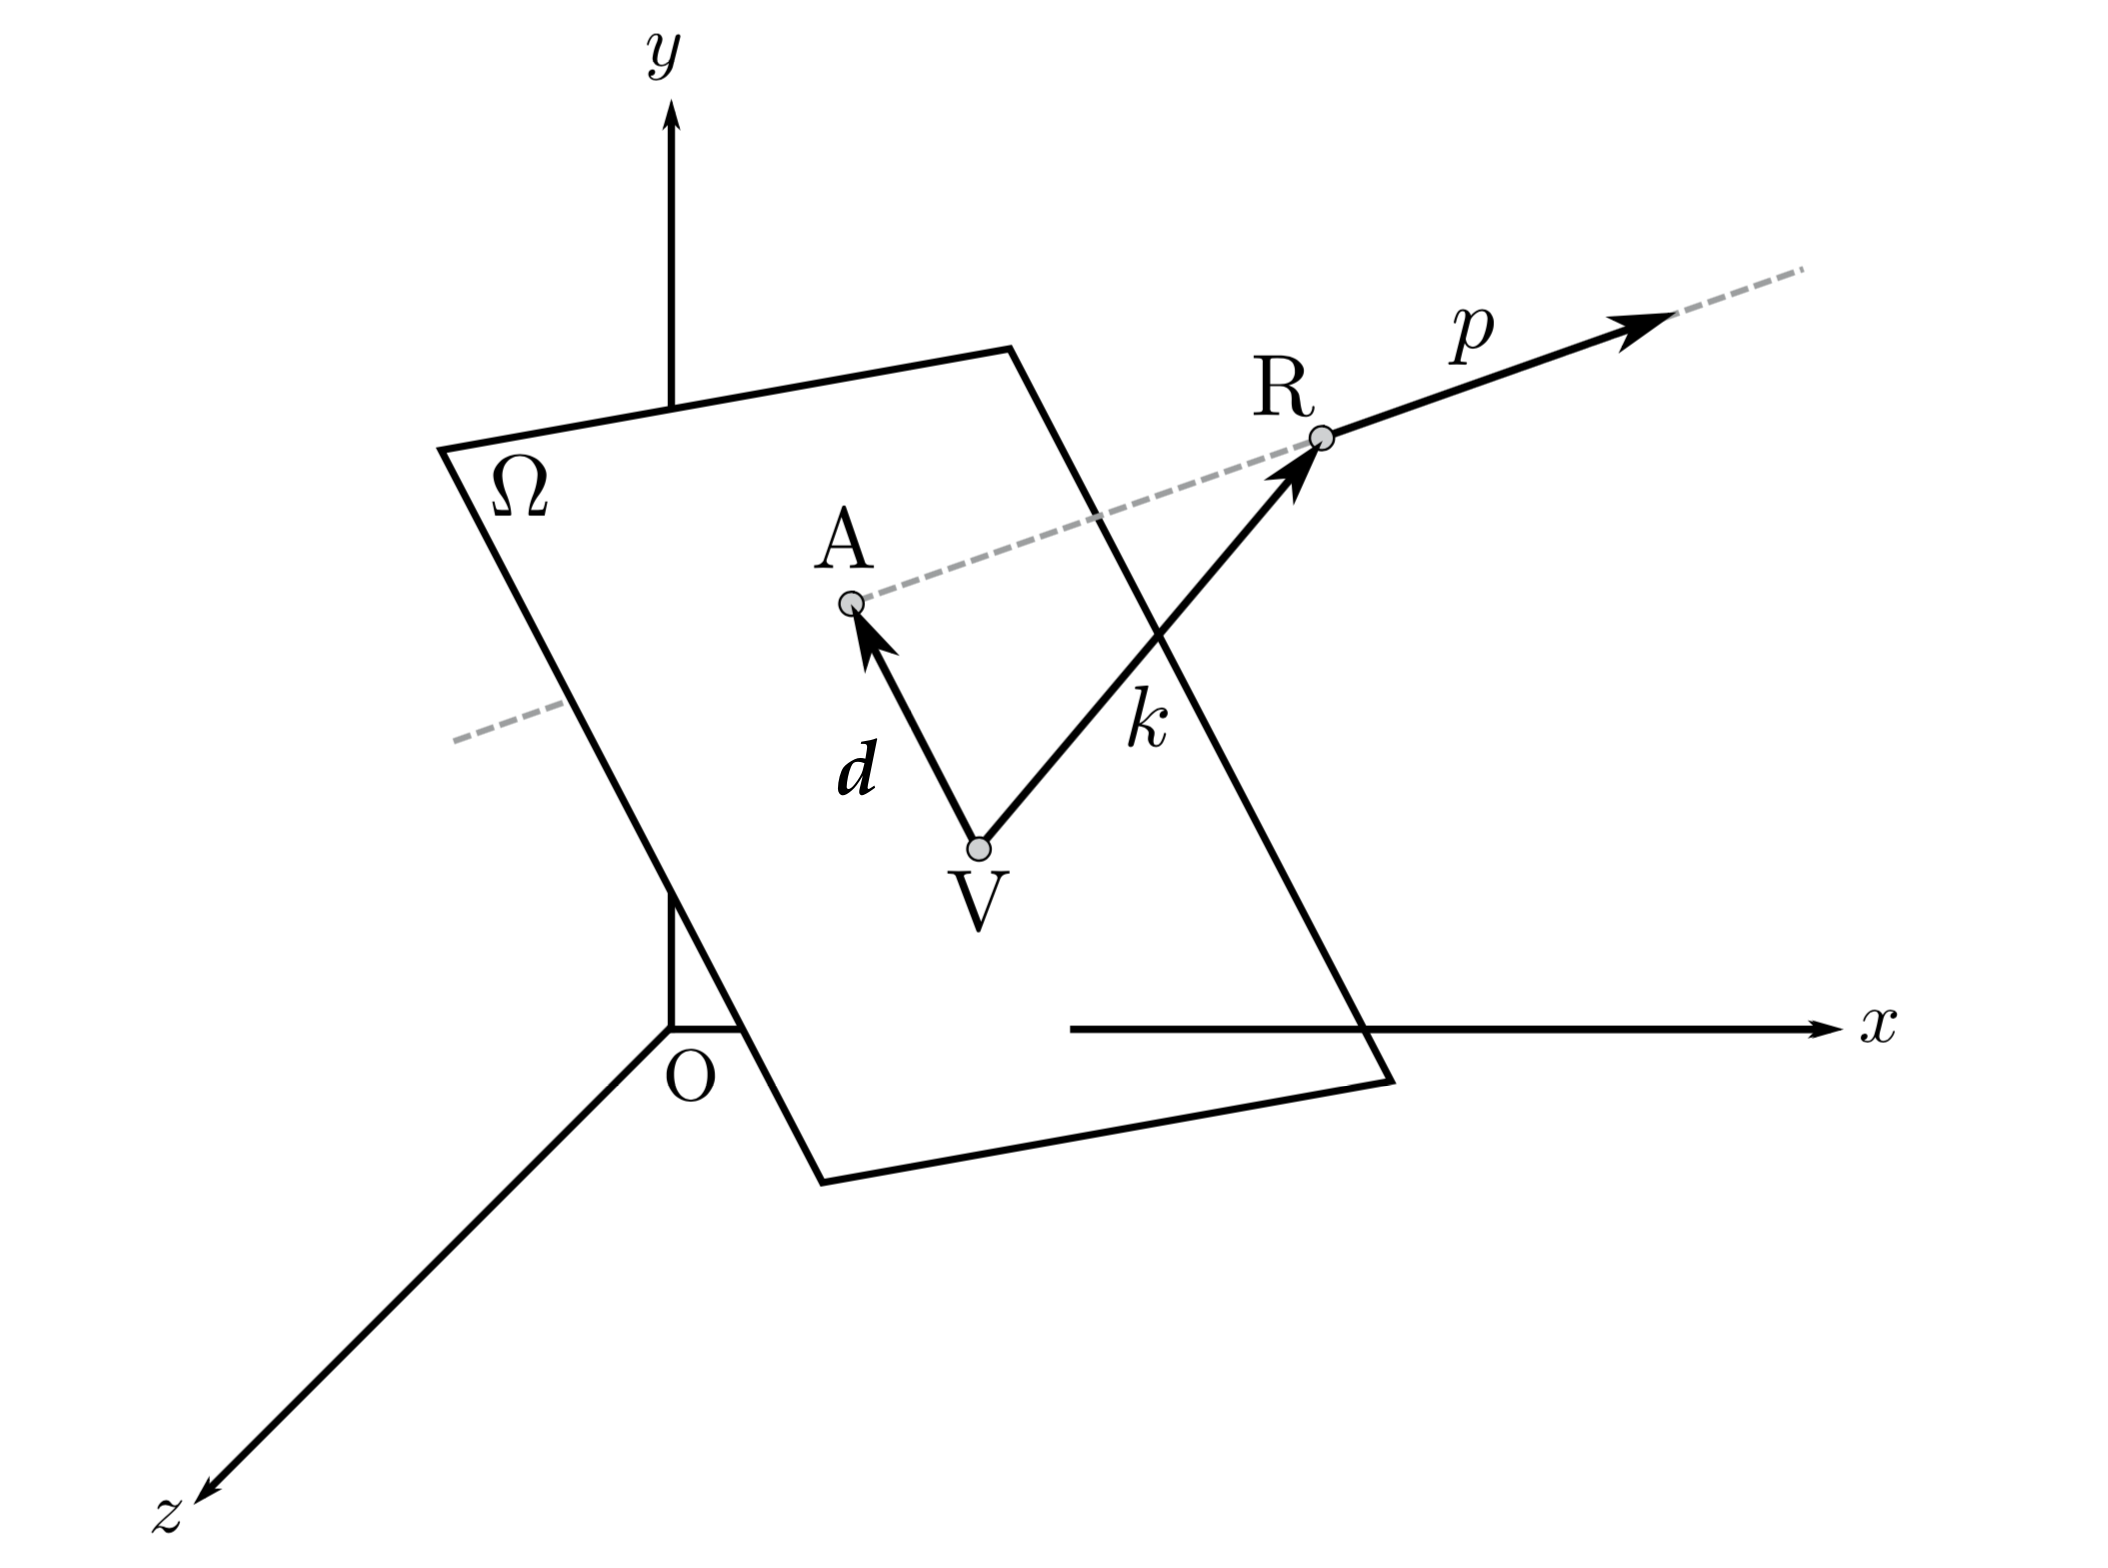
\includegraphics[width=0.7\linewidth]{Figures/IP_tangential_copie}
	\caption{The geometry of finding the IP vector $\boldsymbol{d}$. \parencite{Claudia_thesis}}
	\label{fig:iptangential}
\end{figure}\\
To determine the IP vector with this method, consider Fig. \ref{fig:iptangential}, where V is the primary vertex. From the definition of the impact parameter follows that the distance between the straight line defined by the 3-momentum vector $\boldsymbol{p}$ of the charched child particle at \textbf{R} and the primary vertex point V should be minimised. In other terms, the IP vector $\boldsymbol{d}$ should stay orthogonal to the (normalised) momentum vector $\boldsymbol{\hat{p}}$ meaning
\begin{equation}
	\boldsymbol{d} \cdot \boldsymbol{\hat{p}} = 0.
\end{equation}
The vector $\boldsymbol{d}$ can be expressed using its endpoints $V$ and $A$ as
\begin{equation}
	 \boldsymbol{d} = \overrightarrow{VA} = \boldsymbol{k}+\alpha \cdot \boldsymbol{\hat{p}},
\end{equation}
with $\alpha \in \mathbb{R}$. Combining the two conditions yields
\begin{equation}
	\alpha = -\boldsymbol{k}\cdot\boldsymbol{\hat{p}}
\end{equation}
which then can be used to determine $\boldsymbol{d}$:
\begin{equation}
	\label{ansatz_sol_Claudia}
	\boldsymbol{d} = \boldsymbol{k}-(\boldsymbol{k}\cdot\boldsymbol{\hat{p}})\boldsymbol{\hat{p}}
\end{equation}
There are however multiple problems with such an approach. First, it uses an arbitrarily chosen point \textbf{R} on the helix with no physical meaning to obtain a physical parameter, $\boldsymbol{d}$. Second, it does not take the curvature of the particle trajectory into account, leading to errors. Third, and most importantly, the basic assumption (about the position of the primary vertex being close to the centre of the CMS origin) on which this algorithm lies upon, does not necessarily hold, see Fig. \ref{fig:PVs}. In this figure, one can immediately observe that the position of the primary vertices is of the same order of magnitude as the length of the impact parameter vectors (see Fig. \ref{fig:lambda_dist} in Ch. \ref{Chapter4}). Therefore, a further study of IP reconstruction needs to be considered.\\
\begin{figure}[h]
	\centering
	\subfigure{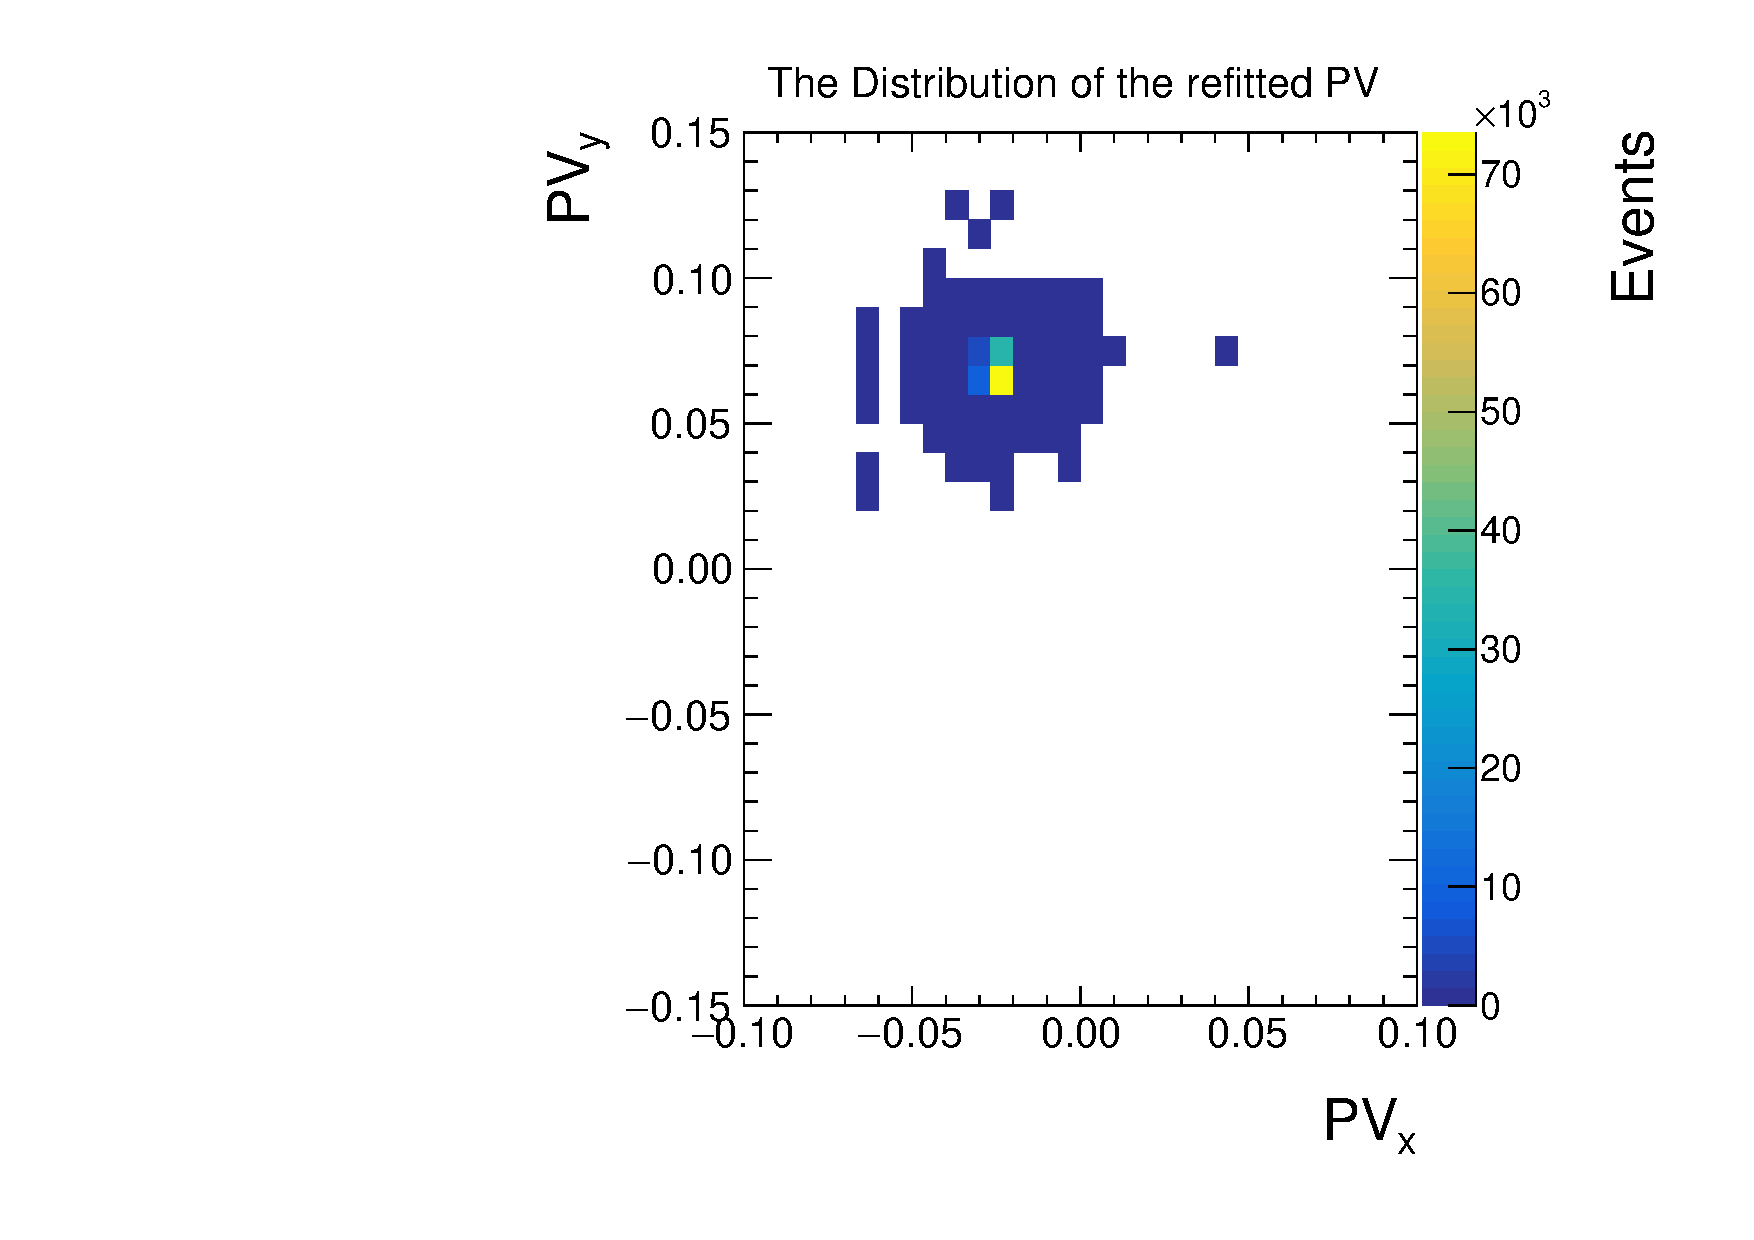
\includegraphics[width=0.4\linewidth]{Figures/PVs}}
	\subfigure{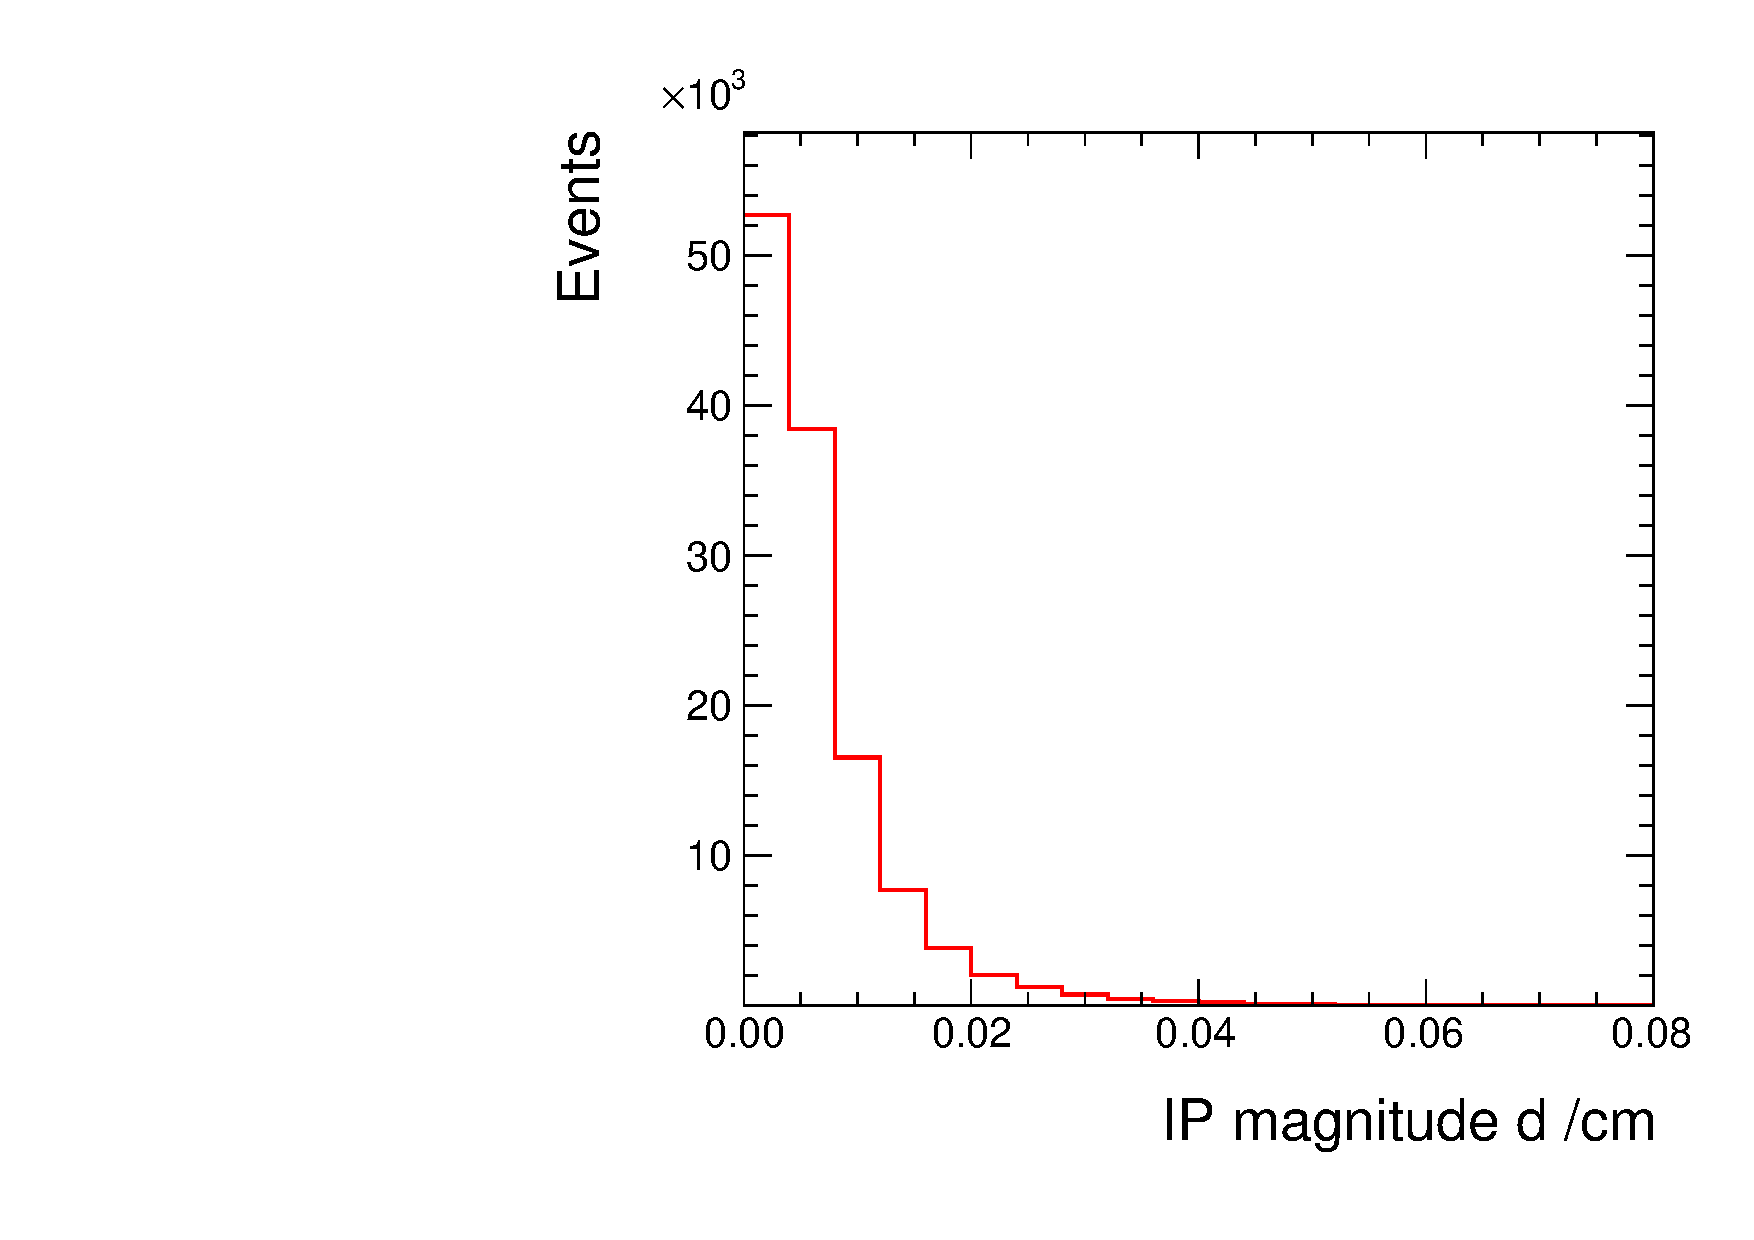
\includegraphics[width=0.4\linewidth]{Figures/IP_mag.pdf}}
	\caption{Left: The positions of the refitted primary vertices of the Higgs decays. Right: The distribution of IP magnitudes in all decay channels. One can observe the distance of the PV from the origin is of the same order of magnitude as the IP length.}
	\label{fig:PVs}
\end{figure}
\newpage
\section{The helical approximation}
Given the fact that both the $\tau$ particles and the secondary vertices cannot be precisely reconstructed, one needs to find a point which lies as closely as possible to the latter. Another assumption (with respect to the tangential approximation) is the consideration of the point of closest approach (PCA) of the particle on its trajectory as the base of IP reconstruction. Having defined the IP vector as the vector pointing from the primary vertex V to the PCA and considering the helix parametrised as in Eq. \ref{eq:ansatz}, it is simple to obtain the newly defined impact parameter, by minimising
\begin{equation}
	\delta(t) = |\boldsymbol{x}(t)-\boldsymbol{v}|^2,
\end{equation}
in $t$, where \textbf{v} denotes the vector pointing from the origin to V. Since $\delta(t)$ is a smooth function with existing higher-order derivatives, the problem can be  calculated numerically.
\subsection{Implementation}
Nevertheless, comparing the fit parameters with Eq. \ref{eq:ansatz}, one first needs to find a bijection between the two parametrisations. However, since both $R$ and $\omega$ are known from the particle's properties, it remains only to determine \textbf{O'}, $\varphi_1 \in [-\pi,\pi)$ and $v_z$.
\paragraph{Finding $\varphi_1$}\mbox{}\\
While determining $\varphi_1$, it has to be taken into consideration that only the $\varphi$-component of the tangent in \textbf{R} is known, from which $\varphi_1$ cannot be easily obtained just by adding or subtracting $\pi/2$. An example of this problem is visualised in Fig. \ref{fig:geometry2}. In this two independent cases portrayed here, one can obtain $\tilde{\varphi_1}$ from $\tilde{\varphi}$ via $\tilde{\varphi_1}=-\tilde{\varphi}+\frac{\pi}{2}$ (keeping the sign convention of Eq. \ref{eq:ansatz} in mind). However, in case of $\hat{\varphi}$ and $\hat{\varphi_1}$ this relation becomes $\hat{\varphi_1} = -\hat{\varphi}$. For this reason, one needs to consider different cases separately.
\begin{figure}[h]
	\centering
	\begin{tikzpicture}
	\centering
	
	\def\centerarc[#1](#2)(#3:#4:#5)% Syntax: [draw options] (center) (initial angle:final angle:radius)
	{ \draw[#1] ($(#2)+({#5*cos(#3)},{#5*sin(#3)})$) arc (#3:#4:#5); }
	
	\draw[thick,->, name path = x_axis_line] (-8,0) -- (5,0) node[anchor=north west] (x_axis) {x};
	\draw[thick,->] (0,-1) -- (0,4) node[anchor=south east] {y};
	\fill (0,0) circle (2pt) node[anchor=north east]{O};


	\centerarc[name path = c](-8,6)(300:350:6);
	\path [name path = Op,draw] (0,0) -- (-8,6) coordinate (Op_point);
	\draw[dashed, name path = horizontal_Op] (-8.5,6)--(-7,6)  coordinate (horizontal_Op_line);
	\fill (-8,6) circle (2pt) node[anchor=south]{$\hat{O'}$};
	\fill [name intersections={of=Op and c}]
	(intersection-1) circle (2pt) node[anchor=west] {$\hat{R}$} coordinate (R);
	\draw[dashed, name path = tangent_line] (intersection-1) --++(-3,-4);
	\draw[dashed] (intersection-1) --++(3,4) coordinate (tangent);
	\draw[line width=0.6mm,->] (intersection-1) --++(0.5,0.66) node [left = 3pt] {$\boldsymbol{\hat{p}}_T$};
	\fill [name intersections={of=tangent_line and x_axis_line}]
	(intersection-1) circle (0pt) coordinate[anchor=north east] (inter);
	\pic [draw, ->, "$\hat{\varphi}$", angle eccentricity=0.6,angle radius=11mm] {angle =x_axis--inter--tangent};
	\pic [draw, <-, "$\hat{\varphi_1}$", angle eccentricity=0.6,angle radius=12mm] {angle = R--Op_point--horizontal_Op_line};
	

	%\draw [name path = c] (8,6) circle (4);
	\centerarc[name path = c](4,3)(170:260:3);
	\path [name path = Op,draw] (0,0) -- (4,3) coordinate (Op_point);
	\draw[dashed, name path = horizontal_Op] (3.5,3)--(5,3)  coordinate (horizontal_Op_line);
	\fill (4,3) circle (2pt) node[anchor=south]{$\tilde{O'}$};
	\fill [name intersections={of=Op and c}]
	(intersection-1) circle (2pt) node[anchor=east] {$\tilde{R}$} coordinate (R);
	\draw[dashed, name path = tangent_line] (intersection-1) --++(2,-2.66) coordinate (tangent);
	\draw[line width=0.6mm,->] (intersection-1) --++(0.5,-0.66) node [left=3pt] {$\boldsymbol{\tilde{p}}_T$};
	\draw[dashed] (intersection-1) --++(-3,4); %(3,-4)
	\fill [name intersections={of=tangent_line and x_axis_line}]
	(intersection-1) circle (0pt) coordinate[anchor=north east] (inter);
	\draw[dashed] (intersection-1) --++(-3,4);
	\pic [draw, <-, "$\tilde{\varphi}$", angle eccentricity=0.6,angle radius=11mm] {angle = tangent--inter--x_axis};
	\pic [draw, <-, "$\tilde{\varphi_1}$", angle eccentricity=0.6,angle radius=5mm] {angle = R--Op_point--horizontal_Op_line};
	\end{tikzpicture}
	\caption{Visualisation of two cases for two different negatively charged particles showing the non-trivial relation between $\varphi_1$ and $\varphi$. Here, $\hat{\varphi_1} = -\hat{\varphi}$ (left case) and $\tilde{\varphi_1}=-\tilde{\varphi}+\frac{\pi}{2}$ (right case).}
	\label{fig:geometry2}
\end{figure}\\
First consider a negatively charged particle following a rotatory trajectory in a positive direction $\varphi$ in the XY-plane. For such a particle, one could rotate the normalised tangent vector at \textbf{R} with $\pi/2$ in the negative rotatory direction and consider the newly constructed radial vector $\hat{\boldsymbol{r}}$. However, the angle between this vector and the x-axis corresponds to the angle $\varphi_1$ we are looking for; in case of a positively charged particle, one could use the "mirrored version" of this method by rotating the tangent vector in the positive direction. Therefore, there are only these two cases to be considered, based on the charge of the particle.
\begin{figure}[h]
	\centering
	\begin{tikzpicture}
		\centering
		
		\def\centerarc[#1](#2)(#3:#4:#5)% Syntax: [draw options] (center) (initial angle:final angle:radius)
		{ \draw[#1] ($(#2)+({#5*cos(#3)},{#5*sin(#3)})$) arc (#3:#4:#5); }
		
		\fill (-7,0) circle (2pt) node[anchor=north east]{O'};
		\draw[dashed] (-7,0)--(-5,0);
		\centerarc[->](-7,0)(0:25:1.5);
		\node at (-6,0.2) {$\varphi_1$};
		
		\centerarc[line width=0.3mm,->](-7,0)(-40:75:4);
		\node[anchor = south west] at ($(-7,0)+({4*cos(75)},{4*sin(75)})$) {\encircle{\textbf{--}}};
		\draw[line width=0.6mm,->] (-7,0)--++($({4*cos(30)},{4*sin(30)})$) node[below = 7pt] {\textbf{R}};
		\draw[line width=0.6mm,->,red] ($({-7+4*cos(30)},{4*sin(30)})$)--++($({-1.5*sin(30)},{1.5*cos(30)})$) node[anchor = south west] {$\hat{p}_T$};
		\draw[dashed, line width=0.6mm,->,red] ($({-7+4*cos(30)},{4*sin(30)})$)--++($({1.5*cos(30)},{1.5*sin(30)})$) node[anchor = south west] {$\hat{r}$};
		\draw[dashed] ($({-7+4*cos(30)},{4*sin(30)})$)--++(1.5,0);
		\centerarc[->]($({-7+4*cos(30)},{4*sin(30)})$)(0:115:0.75);
		\node at ($({-6.9+4*cos(30)},{0.3+4*sin(30)})$) {$\varphi$};
		\centerarc[->]($({-7+4*cos(30)},{0+4*sin(30)})$)(0:28:1.5);
		\node at ($({-6+4*cos(30)},{0.2+4*sin(30)})$) {$\varphi_1$};
		
		\centerarc[line width=0.6mm,->,blue]($({-7+4*cos(30)},{4*sin(30)})$)(120:35:1);
		
		
		\fill (1,0) circle (2pt) node[anchor=north east]{O'};
		\draw[dashed] (1,0)--(3,0);
		\centerarc[->](1,0)(0:25:1.5);
		\node at (2,0.2) {$\varphi_1$};
		
		\centerarc[line width=0.3mm,<-](1,0)(-40:75:4);
		\node[anchor = west] at ($(1,0)+({4*cos(-40)},{4*sin(-40)})$) {\encircle{\textbf{+}}};
		\draw[line width=0.6mm,->] (1,0)--++($({4*cos(30)},{4*sin(30)})$) node[below = 7pt] {\textbf{R}};
		\draw[line width=0.6mm,->,red] ($({1+4*cos(30)},{4*sin(30)})$)--++($({1.5*sin(30)},{-1.5*cos(30)})$) node[anchor = south west] {$\hat{p}_T$};
		\draw[dashed, line width=0.6mm,->,red] ($({1+4*cos(30)},{4*sin(30)})$)--++($({1.5*cos(30)},{1.5*sin(30)})$) node[anchor = south west] {$\hat{r}$};
		\draw[dashed] ($({1+4*cos(30)},{4*sin(30)})$)--++(1.5,0);
		\centerarc[->]($({1+4*cos(30)},{4*sin(30)})$)(0:-55:0.75);
		\node at ($({1.4+4*cos(30)},{-0.3+4*sin(30)})$) {$\varphi$};
		
		\centerarc[->]($({1+4*cos(30)},{4*sin(30)})$)(0:28:1.5);
		\node at ($({2.85+4*cos(30)},{0.3+4*sin(30)})$) {-----$\varphi_1$};
		
		\centerarc[line width=0.6mm,<-,blue]($({1+4*cos(30)},{4*sin(30)})$)(25:-60:1);
		\end{tikzpicture}
	%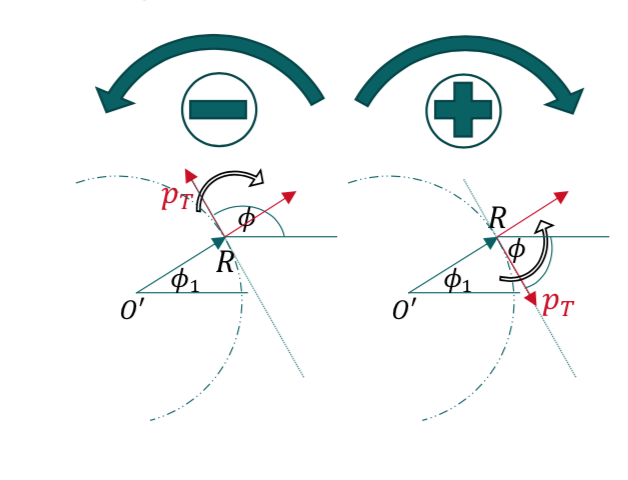
\includegraphics[width=0.7\linewidth]{Figures/rotations.png}
	\caption{Schematic representation of the determination of $\varphi_1$. Here the act of rotation is represented in blue.}
\end{figure}\\
In mathematical terms, let $\hat{\boldsymbol{p}}_T$ be the normalised 3-momentum vector projected to the XY-plane at $t=0$ for a positive particle. Then, the radial vector $\hat{\boldsymbol{r}}$ can be written with the rotation matrix $\textbf{R}_z (\phi)$ for an angle $\phi = \frac{\pi}{2}$ as
\begin{equation}
	\hat{\boldsymbol{r}} = \boldsymbol{R}_z\left(\phi = \frac{\pi}{2}\right)\,\hat{\boldsymbol{p}}_T = \begin{pmatrix}
	0 & -1 \\ 
	1 & 0 
	\end{pmatrix} \begin{pmatrix}
	\cos\varphi\\ 
	\sin\varphi
	\end{pmatrix} = \begin{pmatrix}
	-\sin\varphi\\ 
	\cos\varphi
	\end{pmatrix},
\end{equation}
so that the angle $|\varphi_1|$ between $\hat{\boldsymbol{r}}$ and the x-axis is given by the scalar product
\begin{center}
	\begin{tabular}{crl}
		&$\hat{\boldsymbol{r}} \cdot \boldsymbol{e}_x=$&$ -\sin\varphi= 1 \cdot 1\cdot\cos(|\varphi_1|)$\\
		\rule{0pt}{3ex}$\Rightarrow$&$\varphi_1 =$&$ \arccos(-\sin\varphi)\cdot(-\mathrm{sgn}(\hat{r}_y))$, \\ 
	\end{tabular} 
\end{center}
where the term $(-\mathrm{sgn}(\hat{r}_y))$ is due to the sign convention. Similarly, for a negatively charged particle, this yields
\begin{equation}
	\varphi_1 =\arccos(\sin\varphi)\cdot (-\mathrm{sgn}(\hat{r}_y)).
\end{equation}
The last two equations can be combined to obtain the relation between $\varphi_1$ and $\varphi$:
\begin{equation}
	\varphi_1 =\arccos(-\mathrm{sgn}(q)\sin\varphi)\cdot (-\mathrm{sgn}(\hat{r}_y))
\end{equation}
\paragraph{Finding \textbf{O'}}\mbox{}\\
In order to determine \textbf{O'}, one can use to the arbitrarily introduced parameter $t$ in the ansatz Eq. \ref{eq:ansatz}. Since the location of the particle is completely indifferent from the perspective of the IP problem, one can set the origin of time without any restrictions such that
\begin{equation}
	\boldsymbol{x}(0) = \boldsymbol{O'} +  \left(\begin{tabular}{c}
	$r\cos(\varphi_1) $\\ 
	$-r\sin(\varphi_1) $\\ 
	$0$\\
	\end{tabular} \right) \stackrel{!}{=} \boldsymbol{R}
\end{equation}
yielding
\begin{equation}
	\left\lbrace\begin{tabular}{ll}
	$O'_x =$&$R_x-r\cos(\varphi_1) $\\ 
	$O'_y =$&$R_y+r\sin(\varphi_1) $\\ 
	$O'_z =$&$R_z$\\
	\end{tabular} \right.
\end{equation}
which -- since $\varphi_1$ has already been found as a function of $\varphi$ and \textbf{R} is given by the fit algorithm -- is thereby uniquely defined.
\paragraph{Finding $v_z$}\mbox{}\\
Since the total momentum of the particle is given by $p = m\gamma v$, it follows
\begin{equation}
	v_z = \frac{p}{m\gamma}\cdot\cos\theta = \frac{p}{m\gamma}\cdot\cos\left(\frac{\pi}{2}-\lambda\right) =\frac{p}{m\gamma}\cdot -\sin(-\lambda) =  \frac{p}{m\gamma}\cdot\sin\lambda 
\end{equation}
which can be rewritten using the total energy $E=m\gamma c^2$ of the particle as
\begin{equation}
	v_z = \frac{pc^2}{E} \cdot \sin\lambda = \frac{pc^2}{\sqrt{m^2c^4+p^2c^2}} \sin\lambda = \frac{pc}{\sqrt{m^2c^2+p^2}} \sin\lambda.
\end{equation}
\subsection{Results}
One way of judging the validity of this method is the comparison of the generator level truth with the results obtained by this method on reconstruction level. This has been done in Fig. \ref{fig:deltaphinocut}, where the signed difference between the azimuthal angles $\Delta\phi = \phi(\text{IP}_\text{hel})-\phi({\text{IP}_\text{gen}})$ between the IP on generator level and the IP vectors reconstructed through several methods has been shown. In order to reduce uncertainties when dealing with such minimizer algorithms, this has been done with three different ones: the \verb|TMinimizer| of \verb|ROOT| utilises \verb|Minuit2|, a standard minimizer, secondly, the \verb|Brent|-algorithm, which is a combination of three different numerical minimizer algorithms (the bisection method, the secant method and the inverse quadratic interpolation) and thirdly, an analytical approach which calculates the solution by using a Taylor expansion of the helix for small $\omega t$-values, as discussed in Appendix \ref{AppendixA} (which delivers due to the expansion only approximative information about the overall distribution).
For an algorithm performing better than the current tangential approximation, one expects a narrower distribution concerning $\Delta\phi$, since the algorithm should deliver more reliable results, meaning the reconstructed IP vectors are closer to their generated counterpart. However, this is not the case, no matter which numerical algorithm one considers, therefore errors in the implementation can be excluded. Nevertheless, from the overall form of the distribution follows that there is no major difference between the different minimizer algorithms (\verb|TMinimizer| and \verb|Brent|), except for binning effects, meaning the difference appears only in pairs in two neighbouring bins.\\
While looking at these results, one can also apply the cuts introduced in Chapter \ref{Chapter4}, which is displayed in Fig. \ref{fig:IP_gen_vs_IP_reco}. There are two visible effects of these cuts; firstly, similarly to Fig. \ref{fig:lambdacuts_angles} a disappearance of events with a weakly reconstructed decay plane can observed. Secondly, and more interestingly, the secondary peak around $\Delta\phi \approx -\pi/3$ becomes more visible and more emphasised. This is a clear indicator of systematic deviations in $\Delta\phi$, which arise unsymmetrically. Events of this kind have a reconstructed impact parameter vector which have an angle $\phi(\text{IP}_\text{hel}) \approx \phi(\text{IP}_\text{gen})-\frac{\pi}{3}$ to the generated impact parameter, as shown in Fig. \ref{fig:IP_gen_vs_IP_reco}. In order to judge the capabilities of these algorithms, a more detailed discussion is therefore necessary.
\begin{figure}[h]
	\centering
	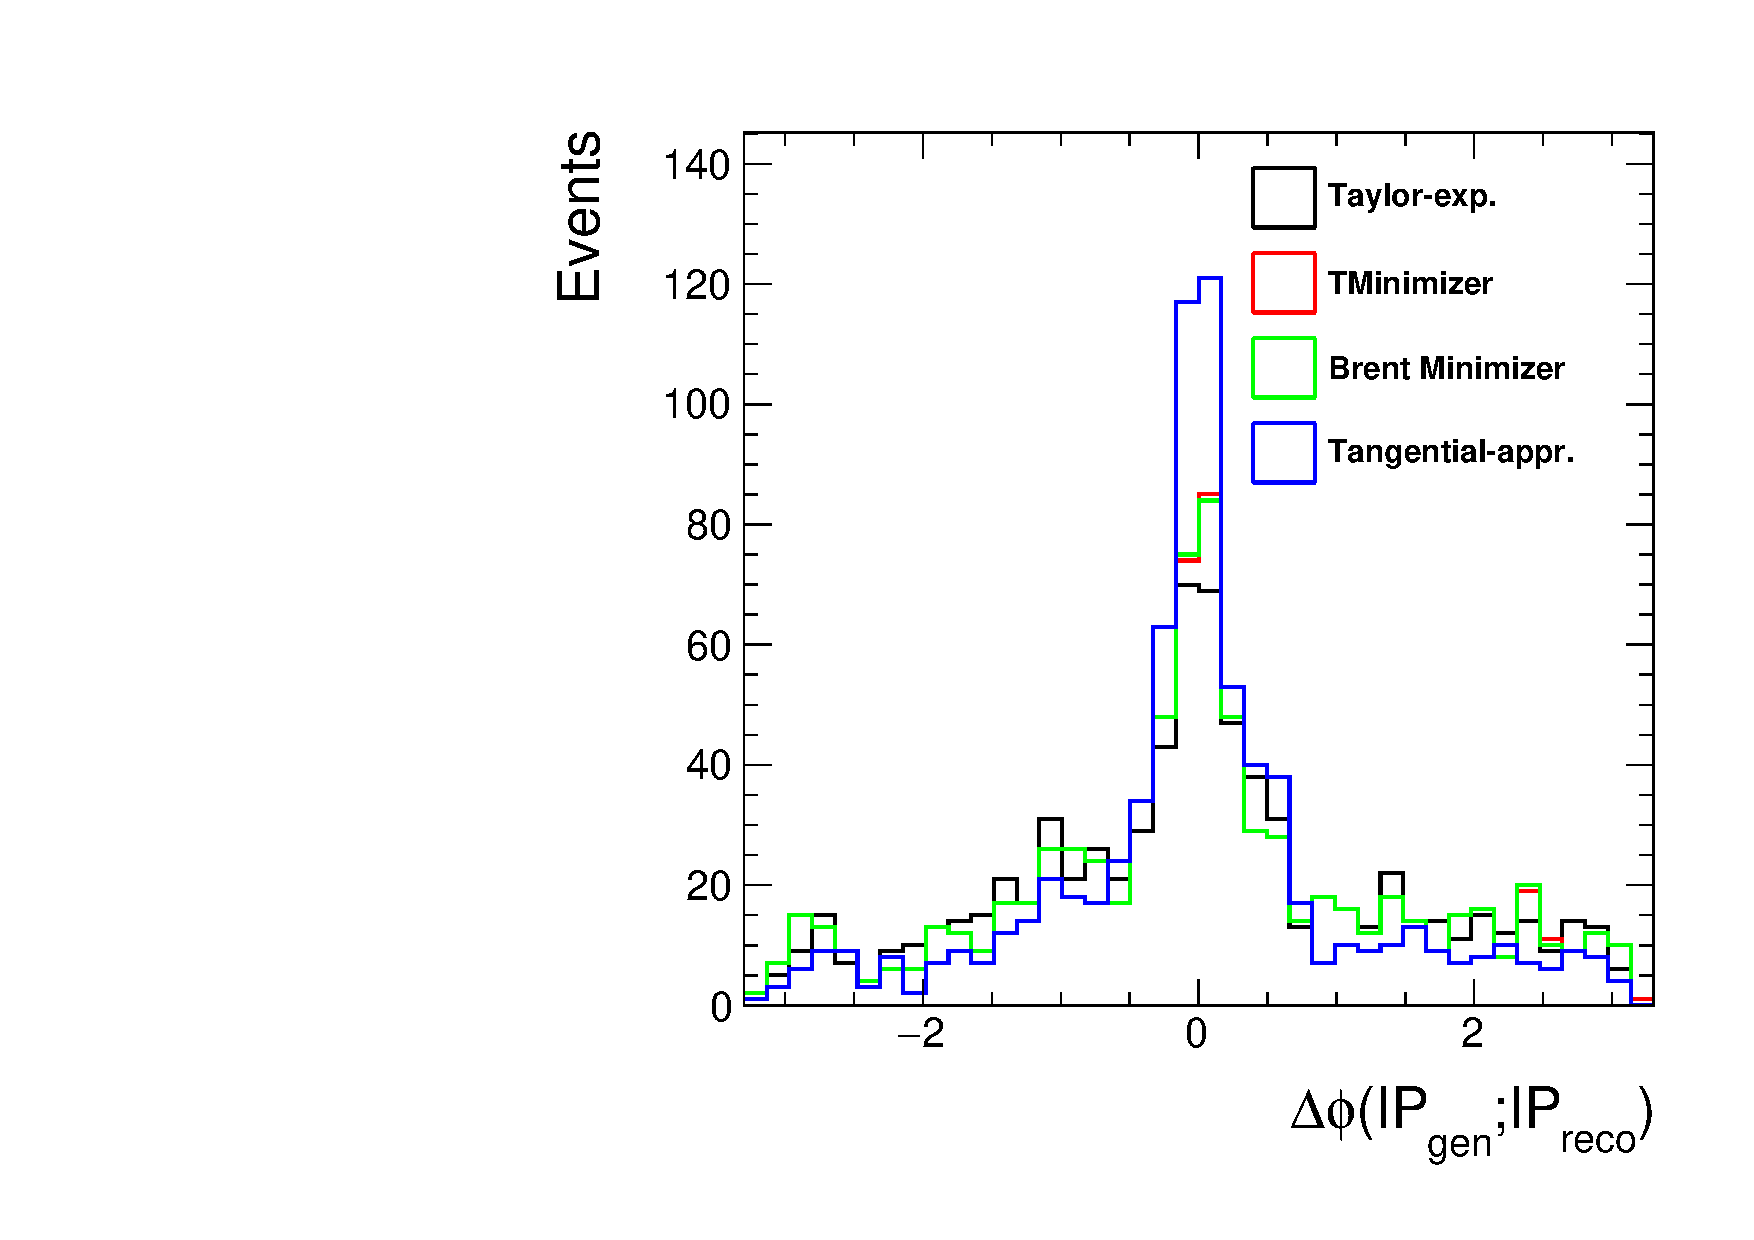
\includegraphics[width=0.7\linewidth]{Figures/deltaPhi_nocut}
	\caption{The comparison of generated and reconstructed IPs by using $\Delta\phi = \phi(\text{IP}_\text{hel})-\phi({\text{IP}_\text{gen}})$. Both the tangential and helical approach deliver similar distributions, albeit the former being seemingly more precise.}
	\label{fig:deltaphinocut}
\end{figure}\\
\begin{figure}[h!]
	\centering
	\subfigure{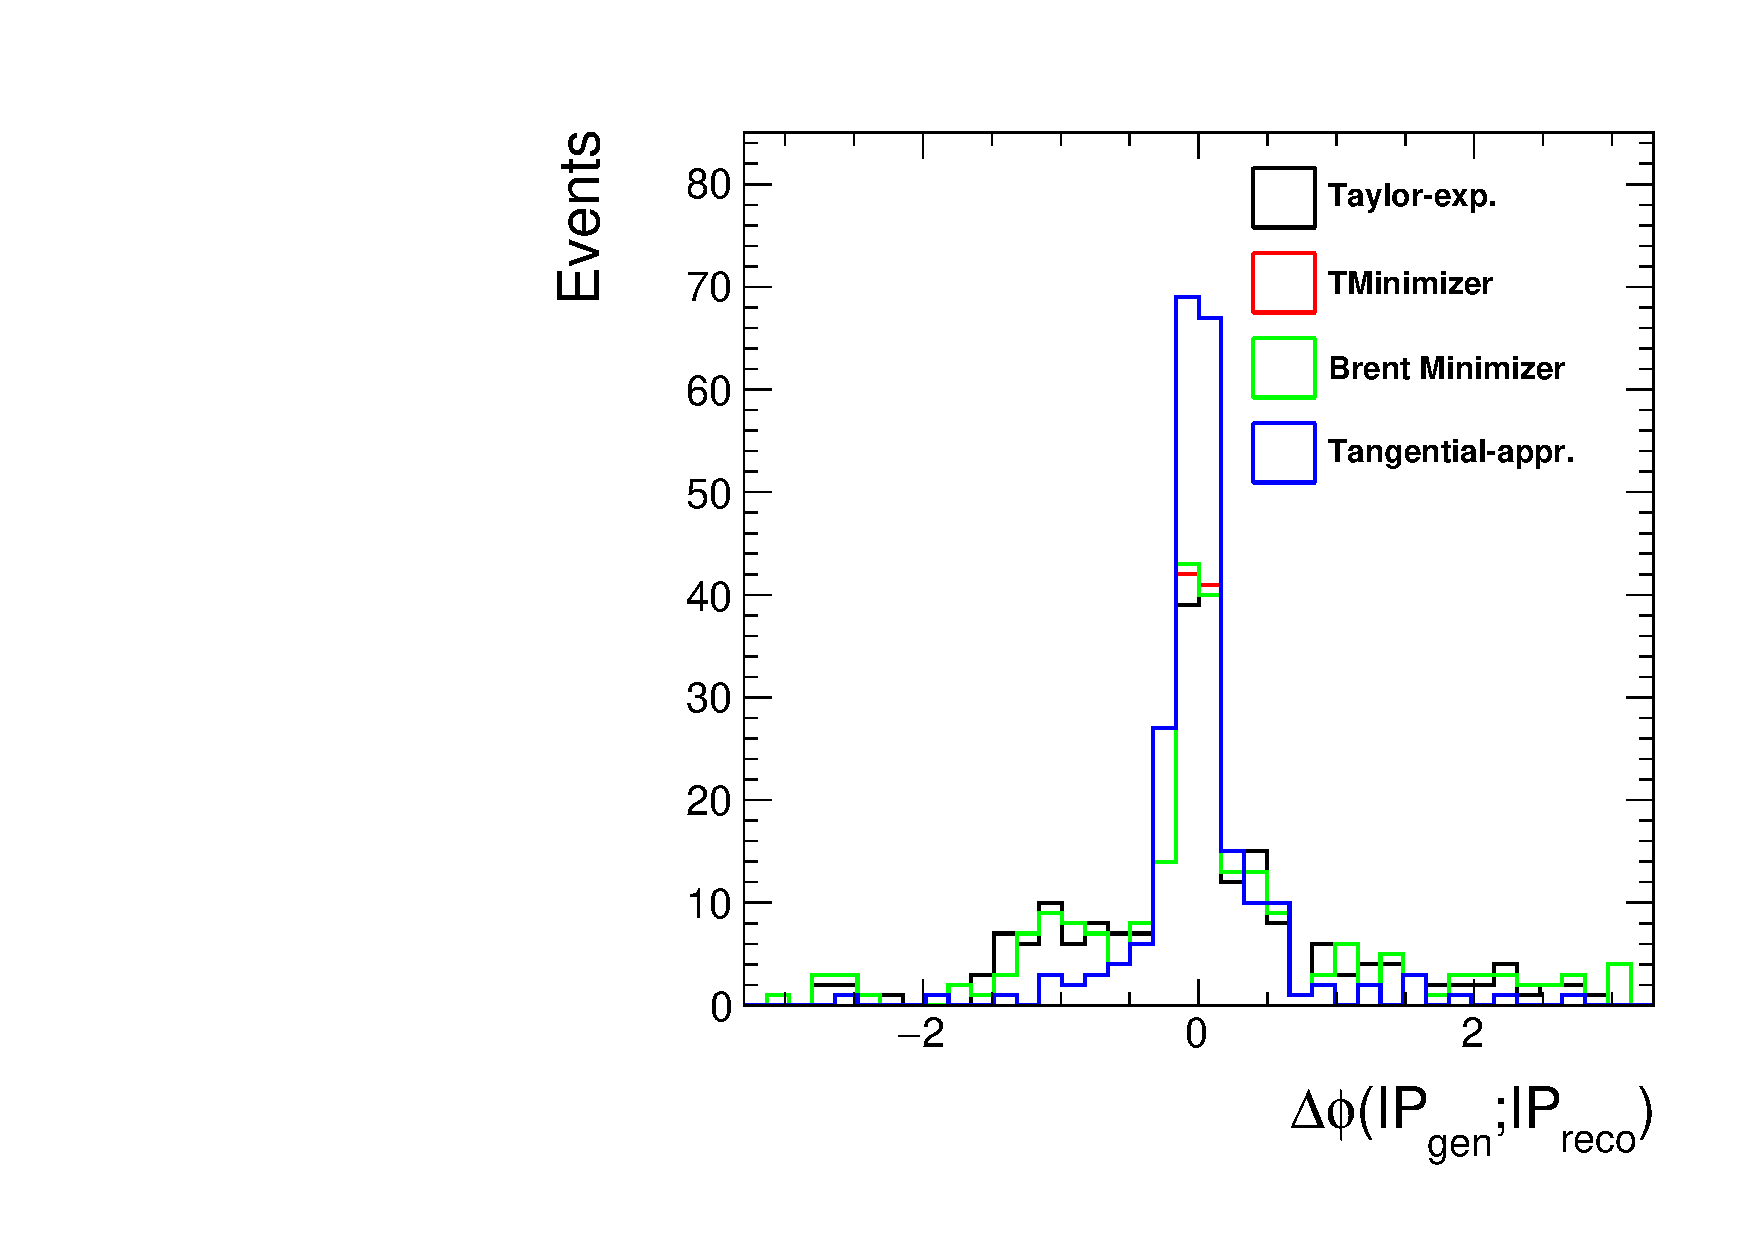
\includegraphics[width=0.5\linewidth]{Figures/deltaPhi_cut}}
	\subfigure{
	\begin{tikzpicture}
	\centering
	\def\centerarc[#1](#2)(#3:#4:#5)% Syntax: [draw options] (center) (initial angle:final angle:radius)
	{ \draw[#1] ($(#2)+({#5*cos(#3)},{#5*sin(#3)})$) arc (#3:#4:#5); }
	
	\path (-2,-3) -- (4,-3);
	\draw[thick,->, name path = x_axis_line] (-1,0) -- (2,0) node[anchor=north west] (x_axis) {x};
	\draw[thick,->] (0,-1) -- (0,2) node[anchor=south west] {y};
	\fill (0,0) circle (2pt) node[anchor=north east]{O};
	
	\draw[thick,->, blue] (0,0) -- (1,1.5) node[anchor=south west] {$\text{IP}_\text{hel}$};
	\node[blue] at (0.5,0.25) {$\phi_1$};
	\centerarc[->, blue](0,0)(0:55:1);
	\draw[thick,->, red] (0,0) -- (-1,2) node[anchor=south east] {$\text{IP}_\text{gen}$};
	\node[red] at (-0.25,1) {$\phi_2$};
	\centerarc[->,red](0,0)(0:116:1.5)
	\end{tikzpicture}}
	\caption{Left: The effect of cuts applied to the distribution of $\Delta\phi$. Here, only events with $d/\sigma_{d} \geq 5$ are kept, whereas a secondary peak at $\Delta\phi \approx -\pi/3$  arises. Right: Schematic representation of the systematic deviations for events with $\Delta\phi = \phi_1-\phi_2\approx -\pi/3$.}
	\label{fig:IP_gen_vs_IP_reco}
\end{figure}\\

\subsection{Discussion of Validity}
In order to interpret and to see the validity of the helical approach, one has to take a look at the projection of the problem to the XY-plane, shown in Fig. \ref{fig:geometry_diffIPs}, where $O$ corresponds to the origin of the coordinate system, \textbf{R} is the vector to the reference point (obtained from the track fit, being the closest point on the trajectory to $O$), $O'$ is the rotation centre of the helical trajectory and PV (SV) denote the primary (secondary) vertices, respectively. In this example, the curvature of the helix is shown in an exaggerated way to emphasize the differences between the different approaches.
\begin{figure}[h]
	\centering
	\begin{tikzpicture}
	\centering
	
	\def\centerarc[#1](#2)(#3:#4:#5)% Syntax: [draw options] (center) (initial angle:final angle:radius)
	{ \draw[#1] ($(#2)+({#5*cos(#3)},{#5*sin(#3)})$) arc (#3:#4:#5); }
	
	\centerarc[<-](0,0)(60:90:8);
	\node[anchor = south] at ($({8*cos(60)},{8*sin(60)})$) {$l$};
	\centerarc[name path = h, dotted,line width=0.3mm, black](0,0)(90:160:8);
	\draw[densely dashed] (-5,8) --(5,8);
	\fill (0,0) circle (2pt) node[anchor=west] {O'};
	\draw[dashed] (0,0) --(0,8) node[anchor = east] at (0,4) {R};
	\fill (0,8) circle (1pt) node[anchor = south] {SV};
	\draw[line width=0.4mm,->] (0,8) -- (3,8) node[anchor=south east] {$p_T$};
	\draw[dashed,line width=0.4mm,->] (-3,5) -- (0,8) node[anchor = west] at (-1.5,6.5) {$\tau$};
	\draw[line width=0.6mm,->] (-3,5) -- (-3,8) node[anchor = west] at (-3,6.5) {$IP_{theo}$};
	\path [name path=OV] (-3,5) -- ++(-3,5);
	\draw [name intersections={of=OV and h, by=x}, ->] [very thick,blue] (-3,5) -- (x) node[below = 10pt] at (x) {$IP_{hel}$};
	\fill ($({6*cos(150)},{6*sin(150)})$) circle (2pt) node[anchor = north] {O};
	\draw[densely dashed, name path=tangent] ($({8*cos(150)},{8*sin(150)})$) --++($({8*sin(150)},{-8*cos(150)})$);
	\draw[dashed] ($({8*cos(150)},{8*sin(150)})$) -- ++ ($({-3*sin(150)},{3*cos(150)})$);
	\draw[line width=0.6mm,->] ($({6*cos(150)},{6*sin(150)})$)--($({8*cos(150)},{8*sin(150)})$)  node[anchor = east] {R};
	\path [name path = V_orth_to_tangent] (-3,5) --++($({6*cos(150)},{6*sin(150)})$);
	\draw [name intersections={of=V_orth_to_tangent and tangent, by=x}, ->] [very thick,red] (-3,5) -- (x) node[left = 1pt] at (x) {$IP_{tan}$};
	\fill (-3,5) circle (2pt) node[anchor=north] {PV};
	\end{tikzpicture}
	\caption{Visualisation of the IPs obtained by different approximations projected to the two-dimensional plane.}
	\label{fig:geometry_diffIPs}
\end{figure}\\
In this graph, one can immediately see that in cases where the primary vertex is far from the origin $O$, the tangential approach becomes physically meaningless as discussed in Ch. \ref{sec:tangential_approx}. In addition, one can see the extreme effect of displacement of the IP vector due to the introduction of the reference point \textbf{R}, the angle between the theoretical and the reconstructed IP having increased. Let alone this would be enough reason to omit the previous approach and to look for an alternative.\\
On the other hand, the fact of ignoring the arbitrarily introduced point \textbf{R} should deliver better results, which should have manifested in a narrower distribution. Nevertheless, the higher peak around 0 in case of the tangential approximation indicates that there are cases where the old method delivers more reliable results. Therefore, a further study and case separation is necessary in order to judge which approximation under which circumstances delivers better results.\\
The root of the problem lies within the fact, that the $\tau$ particles coming from primary vertex can not always be fully reconstructed, or equivalently, the secondary vertex can only be reconstructed at the cost of great uncertainties and only in 3-prong decay channels. For these cases, one could also execute a kinematical fit with respect to the $\tau$ leptons in order to determine the location of the SV, from which, by minimizing the distance between the PV and the tangent defined by the 3-momentum of the child particles, the correct IP vector can be obtained.\\
Another workaround for this problem would be the consideration of electron-positron collisions. In such systems, unlike in case of proton-proton collisions the ZMF is known, since it is not the patrons of the system which interact but the ``pure'' electrons. During a such reaction, the Higgs boson can be produced through the Higgsstrahlung process\\
\begin{figure}[h]
	\centering
	\feynmandiagram [horizontal=a to b] {
		i1[particle=$e$] -- [fermion] a -- [fermion] i2[particle=$e$],
		a -- [photon,edge label=$Z$] b,
		f1[particle=$Z$] -- [photon] b -- [dashed] f2[particle=$H$],
	};
	\caption{Higgs production in electron-positron collisions}
\end{figure}\\
which needs at least a CM-energy of 215 GeV. In order to achieve such energy scales, new colliders are currently planned. However, both solutions go beyond the scope of this thesis.